\documentclass{standalone}

\usepackage{tikz}
\usepackage{circuitikz}

\tikzset{block/.style = {draw, fill=white, very thick, rectangle, minimum height=1cm, minimum width=2cm},
         lblock/.style={draw,fill=white,very thick, rectangle, minimum height=3cm, minimum width=1cm},
         sum/.style= {draw, fill=white, very thick, circle, node distance=0.5cm}}

         
\begin{document}
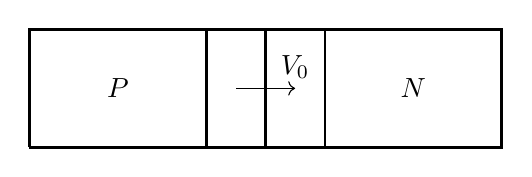
\begin{tikzpicture}[scale=1.5]
    \draw[very thick](-2,0)--(2,0)--(2,1)--(-2,1)--(-2,0);
    \draw[very thick](0,0)--(0,1);
    \draw[thick](0.5,0)--(0.5,1);
    \draw[thick](-0.5,0)--(-0.5,1);

    \node at (1.25,0.5) {$N$};
    \node at (-1.25,0.5) {$P$};

    \draw[->](-0.25,0.5)--(0.25,0.5)node[above]{$V_0$};
\end{tikzpicture}
\end{document}